Computer vision is an important and maturing engineering science. It underpins an increasing variety of applications that require the acquisition, analysis, and interpretation of visual information.

\subsubsection{Feature extraction}
When working with images, it is usually not possible to work with the raw image data itself (the pixel values). The reason for this is the high dimensionality of images, which can easily exist in a space of more than a million dimensions. By extracting features from images, they can be represented in a lower dimensional feature-space.  This feature extraction process has several advantages:
\begin{itemize}
\item The data becomes computationally easier to work with due to the smaller number of dimensions
\item By using the right features, the data becomes more suitable for generalization across images
\item Reducing the dimensionality makes it easier to visualize sets of images
\item Features can have an intuitive basis, which makes it easier for non-computer-scientists to analyze (sets of) images
\end{itemize}

In the extraction of image features, a distinction was made between low-level statistical features and higher level cognitive-based features.

\paragraph{\textit{Statistical features}}
As statistical features, many relatively simple low-level features were extracted from the images.
The first type of statistical features that were used are color-based features, which should capture the color-usage in the artwork. Many artists produce collections of art pieces with similar colors, and should therefore be (partially) distinguishable with color-based features. For each of the three RGB channels, an average and median is calculated over all the channel values. Let $\{\mathbf{x}_{m,i,c} \}_{i=1\dots n}$ be the pixel values for image $m$ in color channel $c \in \{R,G,B \}$. The average in channel $c$ of image $m$ is then given by 

\begin{equation}
\label{avgChannel}
\mu_c(\mathbf{x}_{m}) = \frac{1}{n}\sum_{i=1}^{n} \mathbf{x}_{m,i,c} 
\end{equation}
The median in channel $c$ is given by 
\begin{equation}
\label{medChannel}
\tilde{\mathbf{x}}_{m,c} = \mathbf{x'}_{m,k,c}
\end{equation}
where $\{\mathbf{x'}_{m,i,c}\}_{i = 1\dots n}$ are the sorted pixel values of channel $c$ and $k = \mbox{round}(n/2)$.
The image is also converted into the HSV color space, from which the average and median is extracted for each channel as defined in equations \ref{avgChannel} and \ref{medChannel}. The Hue channel is given by: 

$H_{m,i} = \left\{ 
\begin{array}{ll}
0 & \mbox{if $C_{m,i} = 0$};\\
60 \left(\frac{G_{m,i}-B_{m,i}}{C_{m,i}} \mbox{mod} 6 \right) & \mbox{if $M_{m,i} = R_{m,i}$};\\
60 \left(\frac{B_{m,i}-R_{m,i}}{C_{m,i}} + 2 \right) & \mbox{if $M_{m,i} = G_{m,i}$};\\
60 \left(\frac{R_{m,i}-G_{m,i}}{C_{m,i}} + 4 \right) & \mbox{if $M_{m,i} = B_{m,i}$}; \\
\end{array} sub
\right\}$
Where $M_{m,i} = \max(R_{m,i},G_{m,i},B_{m,i})$ and $C_{m,i} =  M - \min(R_{m,i},G_{m,i},B_{m,i})$. The value channel is given by $V_{m,i} =  M_{m,i}$ and the saturation channel is  by $S_{m,i} = \frac{C_{m,i}}{V_{m,i}}$

The second group of features is the edge to pixel and corner to pixel ratio. Let $\{\mathbf{x}_{m,i} \}_{i=1\dots n}$ be the pixel values of the binary edge-image produced by applying a Canny edge detector[REF] on image $m$. The edge to pixel ratio of image $m$ is then computed as $f_{e,m} = \frac{1}{n}\sum_{i=1}^{n} \mathbf{x}_{m,i} $. Let $\{\mathbf{y}_{m,i} \}_{i=1\dots n}$ be the pixel values in the binary corner image produced by a corner detector that are either $1$ if the pixel is a corner or $0$ otherwise. The corner to pixel ratio of image $m$ is then computed as  $f_{c,m} = \frac{1}{n}\sum_{i=1}^{n} \mathbf{y_{m,i}} $. These two features should be helpful in distinguishing many photography artworks from other genres such as cartoons and manga. The latter two tend to have large patches of plain color patches, which will decrease the amount of edges and corners. They are also somewhat indicative to the type of scenes in photography. A blue sky will not produce many edges or corners, whereas a busy street will.  

%$v : R^2 \rightarrow \{0,1\}$
%calculated by performing Canny edge detection on the image to construct an image of edges. The number of edge pixels in this image, divided by the total number of pixels is then used as a feature. The same is done using a corner detector. 

For the final group of features, the artworks are converted from RGB image $m$ to a greyscale intensity image $I_m$ by taking for each pixel $i$, a weighted sum of the R,G and B channels: $I_{m,i} = 0.2989R_{m,i} + 0.5870G_{m,i} + 0.1140B_{m,i} $. Let $\{\mathbf{z}_{m,i}\}_{i=1\dots n}$ be the pixel values of the greyscale intensity image of image $m$. The average intensity feature is then calculated as $f_{\mu_{I_m}} = \frac{1}{n} \sum_{i = 1}^{n} \mathbf{z}_{m,i}$ and the median intensity as $\tilde{I}_m = \mathbf{z'}_{m,k}$, where $\{\mathbf{z'}_{m,i}\}_{i = 1\dots n}$ are the sorted pixel values and $k = \mbox{round}(n/2)$. These values give information about the lightness or darkness of artworks. The intensity variance feature is computed as $\mbox{Var}(I_m) = \frac{1}{n} \sum_{i=1}^n \mathbf{z}_{m,i}$, which reacts to the contrast between lightness and darkness in images. Finally the entropy of the intensity is calculated as follows. $H(I_m) = -\sum_{u = 1}^{j} \hat{p}_u \log_2(\hat{p}_u) $, where $\{\hat{p}_u(\mathbf{z}_m)\}_{u = 1 \dots j}$ are the histogram bins of the intensity values and are defined as $\hat{p}_u(\mathbf{z}_m) = \sum_{i=1}^n \delta[b(\mathbf{z}_{m,i}) - u] $. The function $b : R \rightarrow \{1 \dots j \}$ returns the index of the bin of the input pixel value in the intensity space and $\delta[g] = 1$ if $g = 0$, otherwise $0$. This feature somewhat characterizes the texture in an image. Figure \ref{featureImg} shows the intermediate representations of an image for different types of features. 

\begin{figure}[!h]
  \begin{center}
    \subfigure[Original image]{\label{centersample}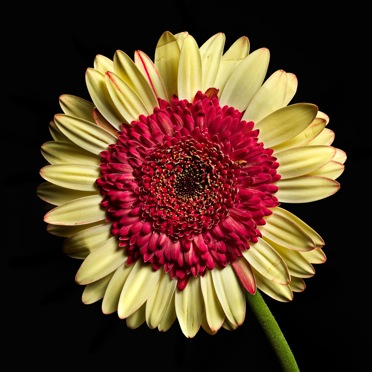
\includegraphics[scale=0.22]{img/originalFlower}}
     \subfigure[Edges]{\label{lssample}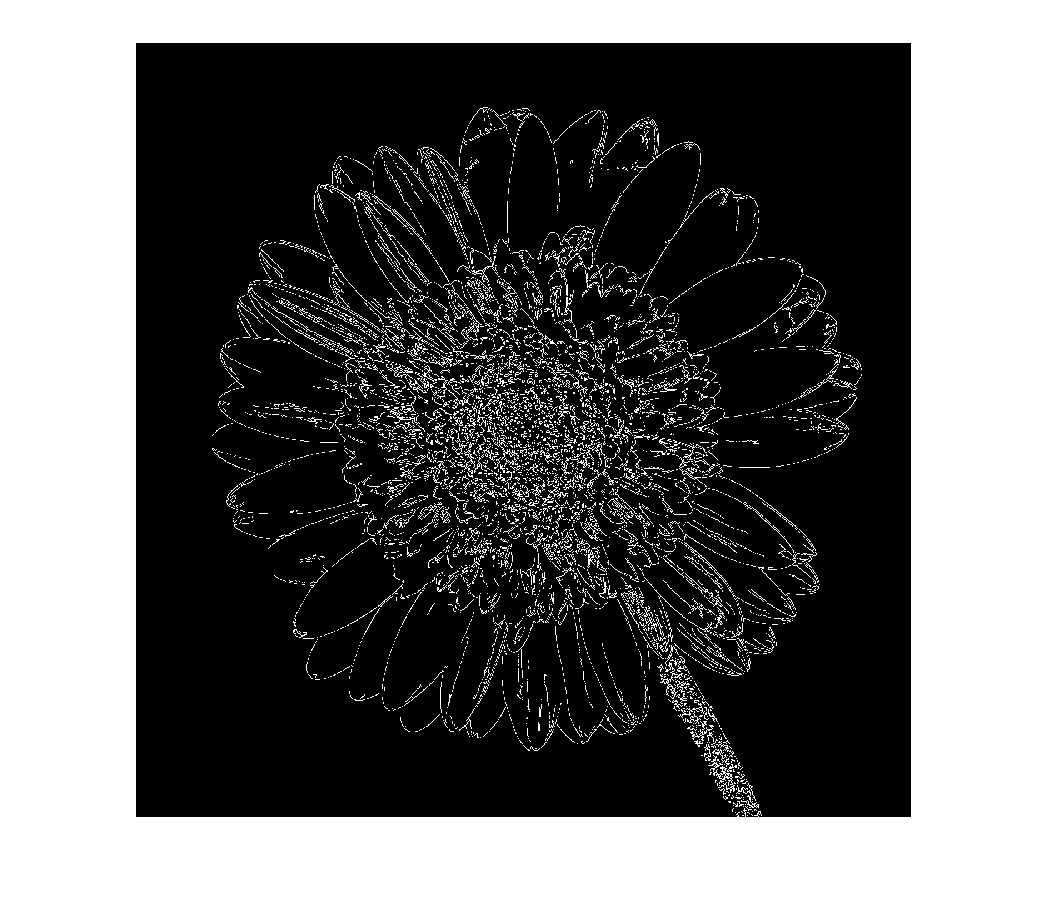
\includegraphics[scale=0.22]{img/edgesFlower}} 
     \subfigure[Corners]{\label{lssample}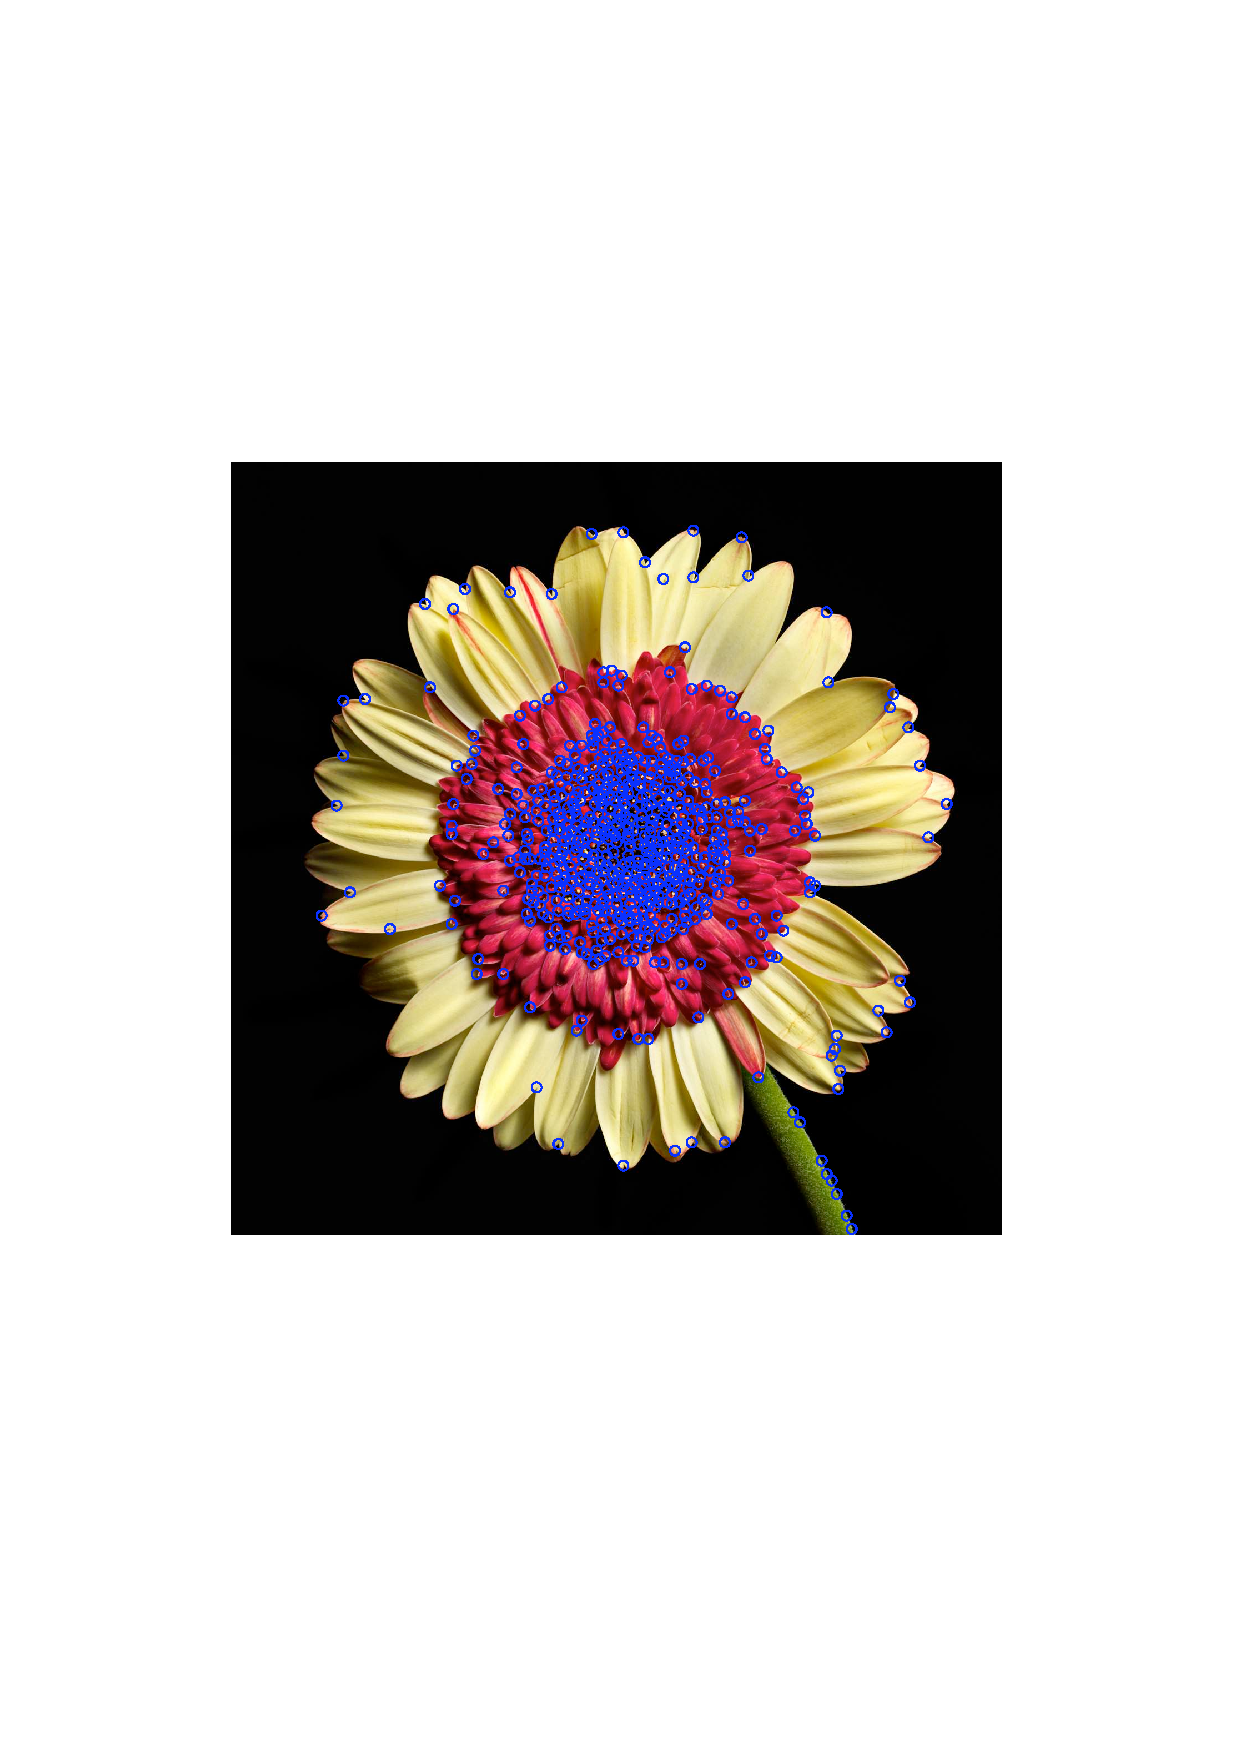
\includegraphics[scale=0.22]{img/cornersFlower}}  
     \subfigure[Hue]{\label{lssample}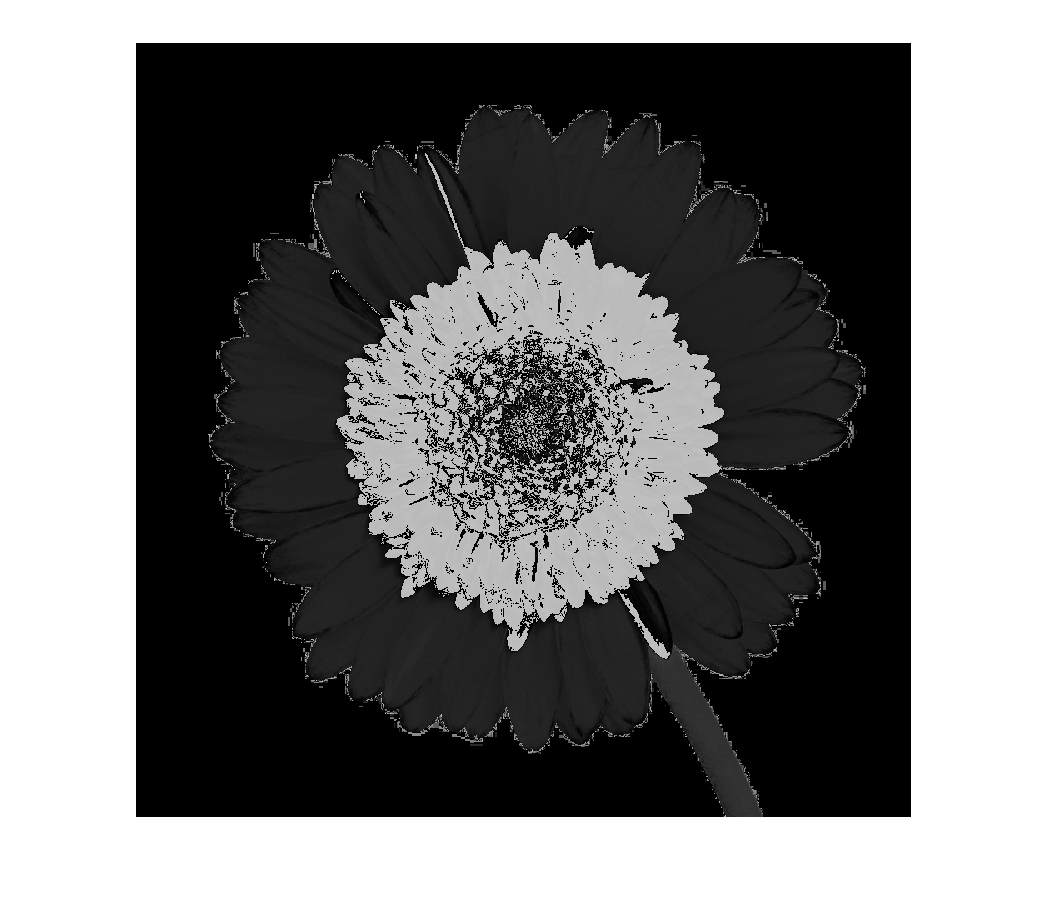
\includegraphics[scale=0.22]{img/hueFlower}}           
     \subfigure[Saturation]{\label{lssample}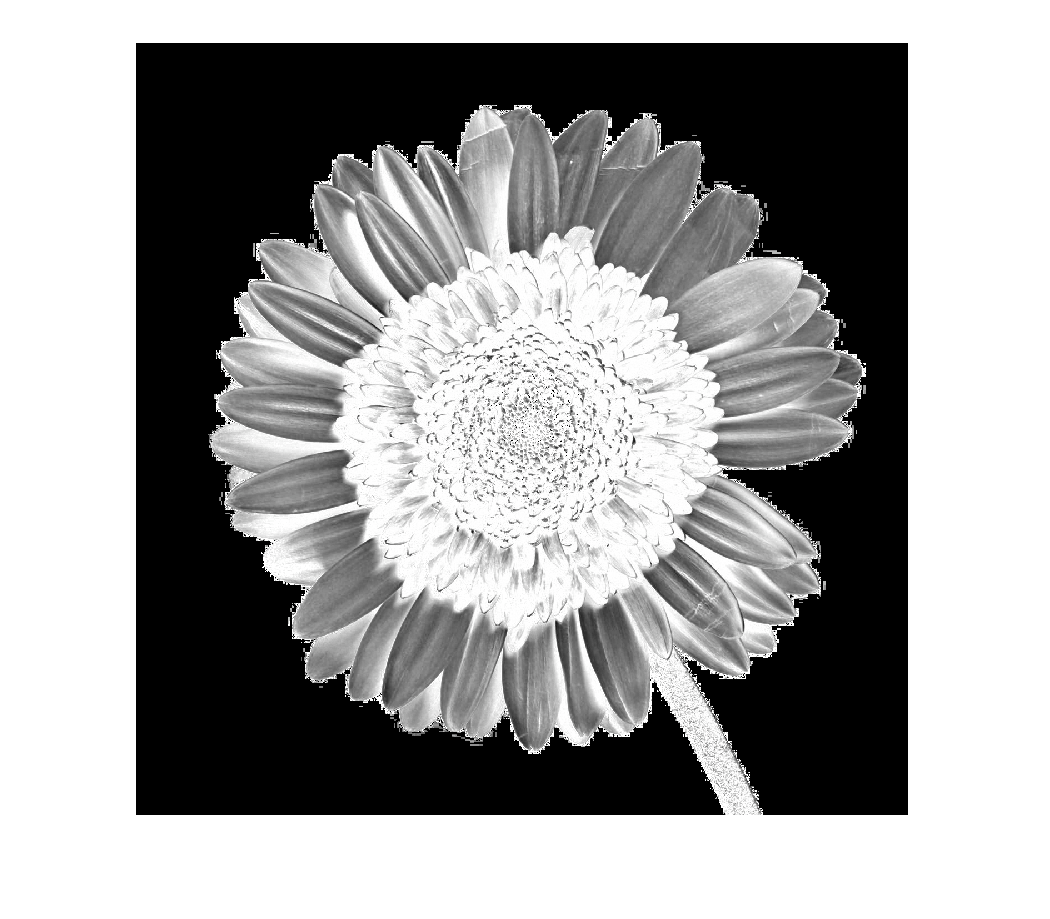
\includegraphics[scale=0.22]{img/satFlower}}           
     \subfigure[Value]{\label{lssample}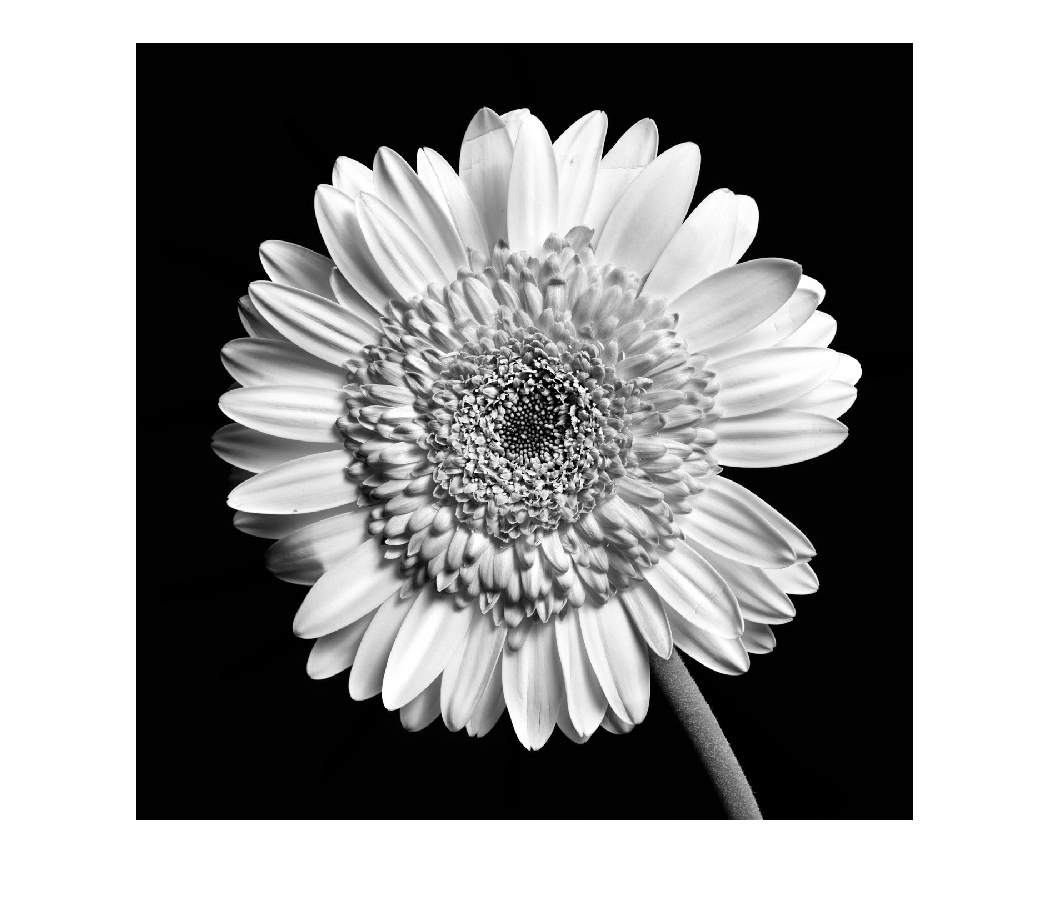
\includegraphics[scale=0.22]{img/valueFlower}}
     \subfigure[Intensity]{\label{lssample}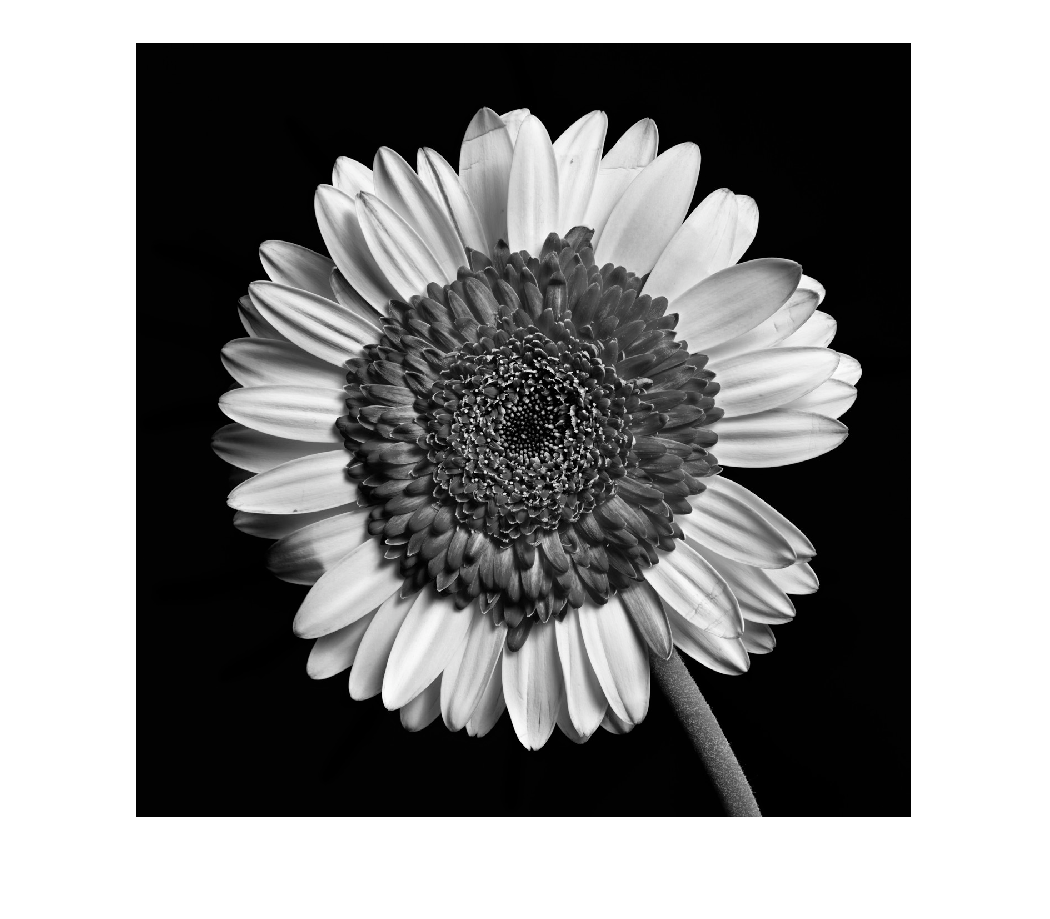
\includegraphics[scale=0.22]{img/intFlower}}                               
     \subfigure[Red]{\label{lssample}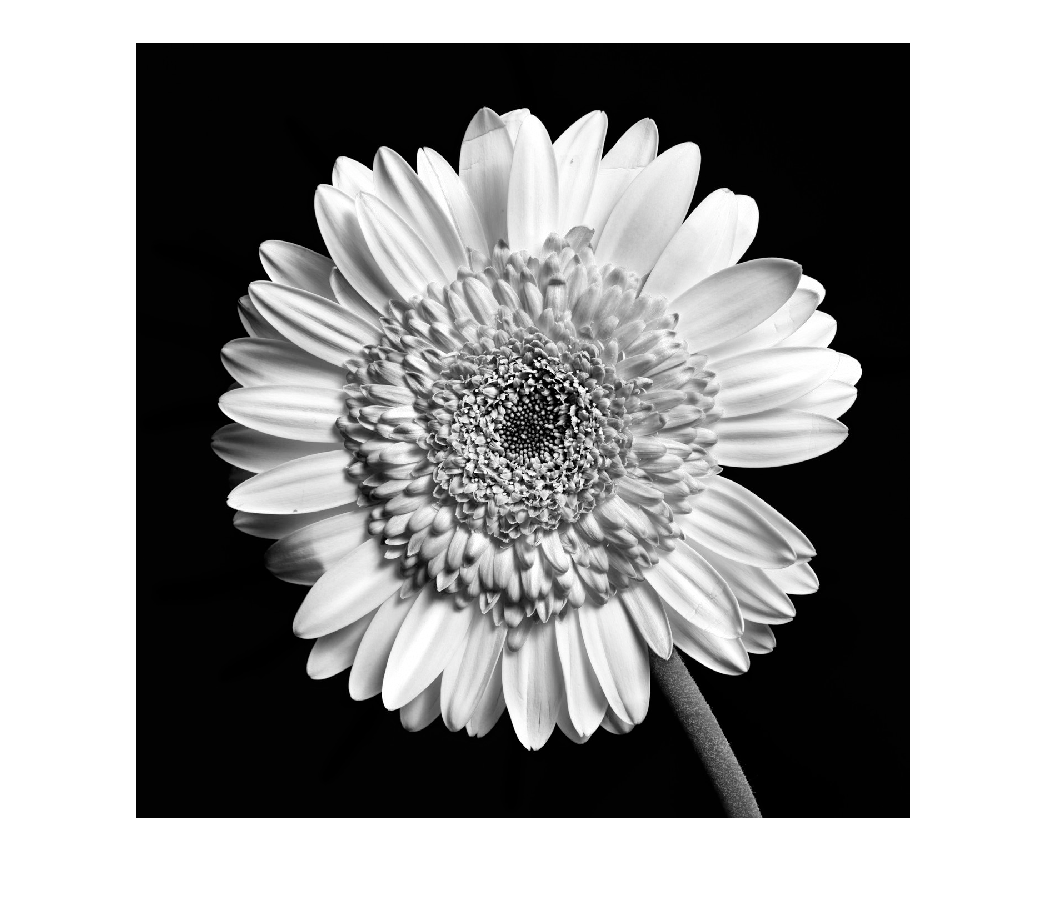
\includegraphics[scale=0.22]{img/redFlower}}
     \subfigure[Green]{\label{lssample}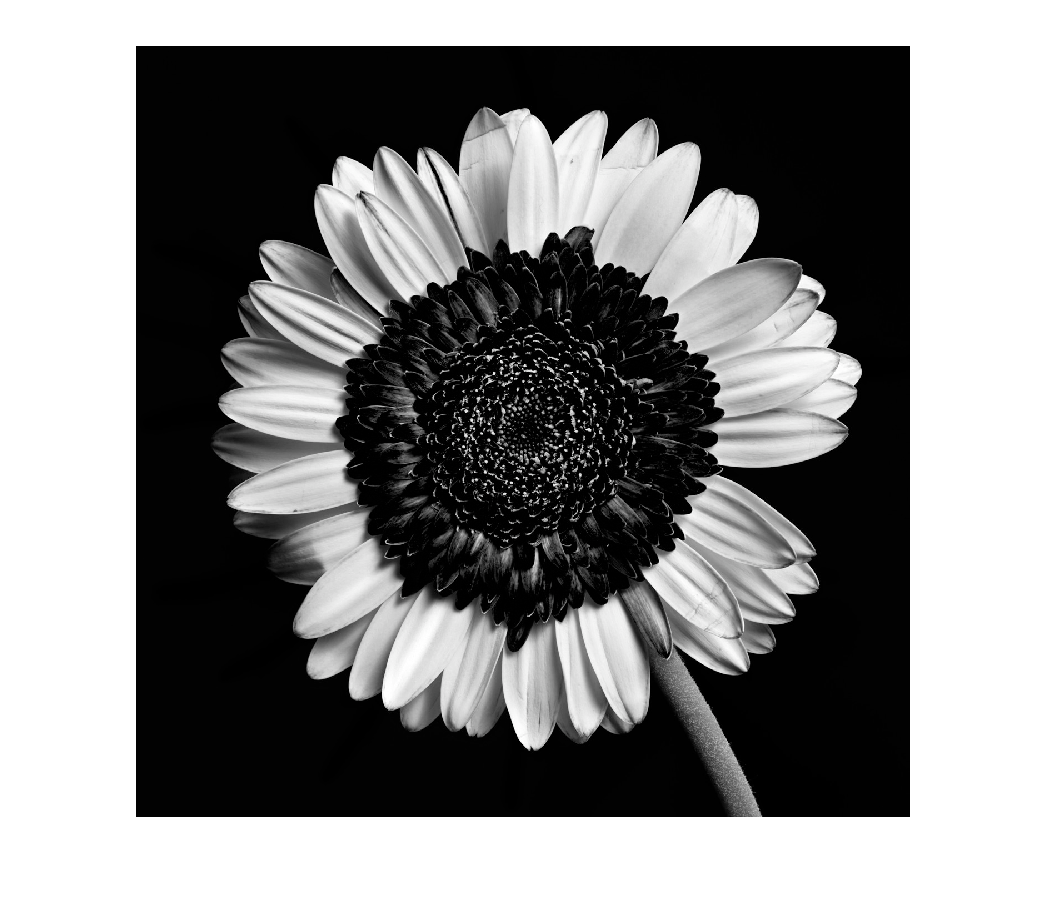
\includegraphics[scale=0.22]{img/greenFlower}}
     \subfigure[Blue]{\label{lssample}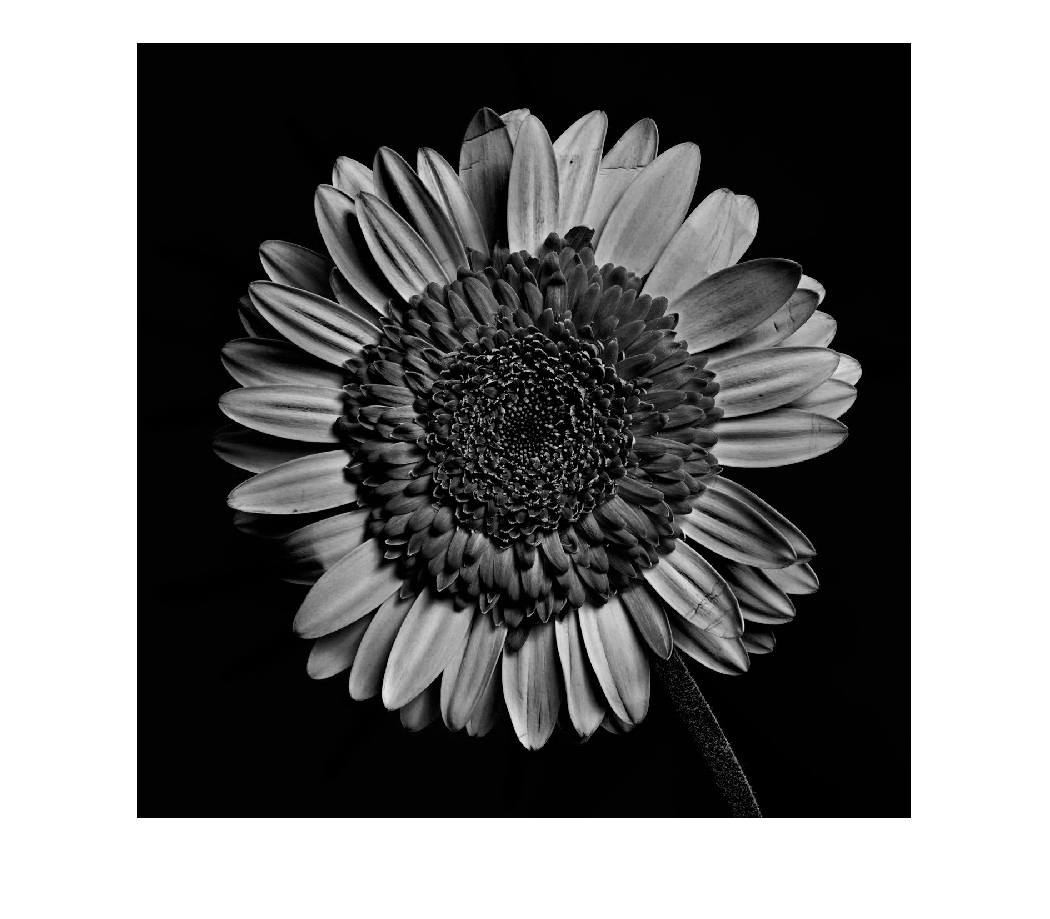
\includegraphics[scale=0.22]{img/blueFlower}}

  \end{center}
  \caption{Illustration of different statistical features}
  \label{featureImg}
\end{figure}


The features described above only contain global information about images. In order to capture localized information as well, several of the features described above are also extracted from different regions of the image. The regions of the image are obtained by dividing the image along both dimensions into NxM equal-sized regions. Since feature values will most likely vary from region region, these compositional features should provide valuable additional information about an image. Figure \ref{gridImage} shows an example of 

\begin{figure}
\label{gridImage}
\begin{center}
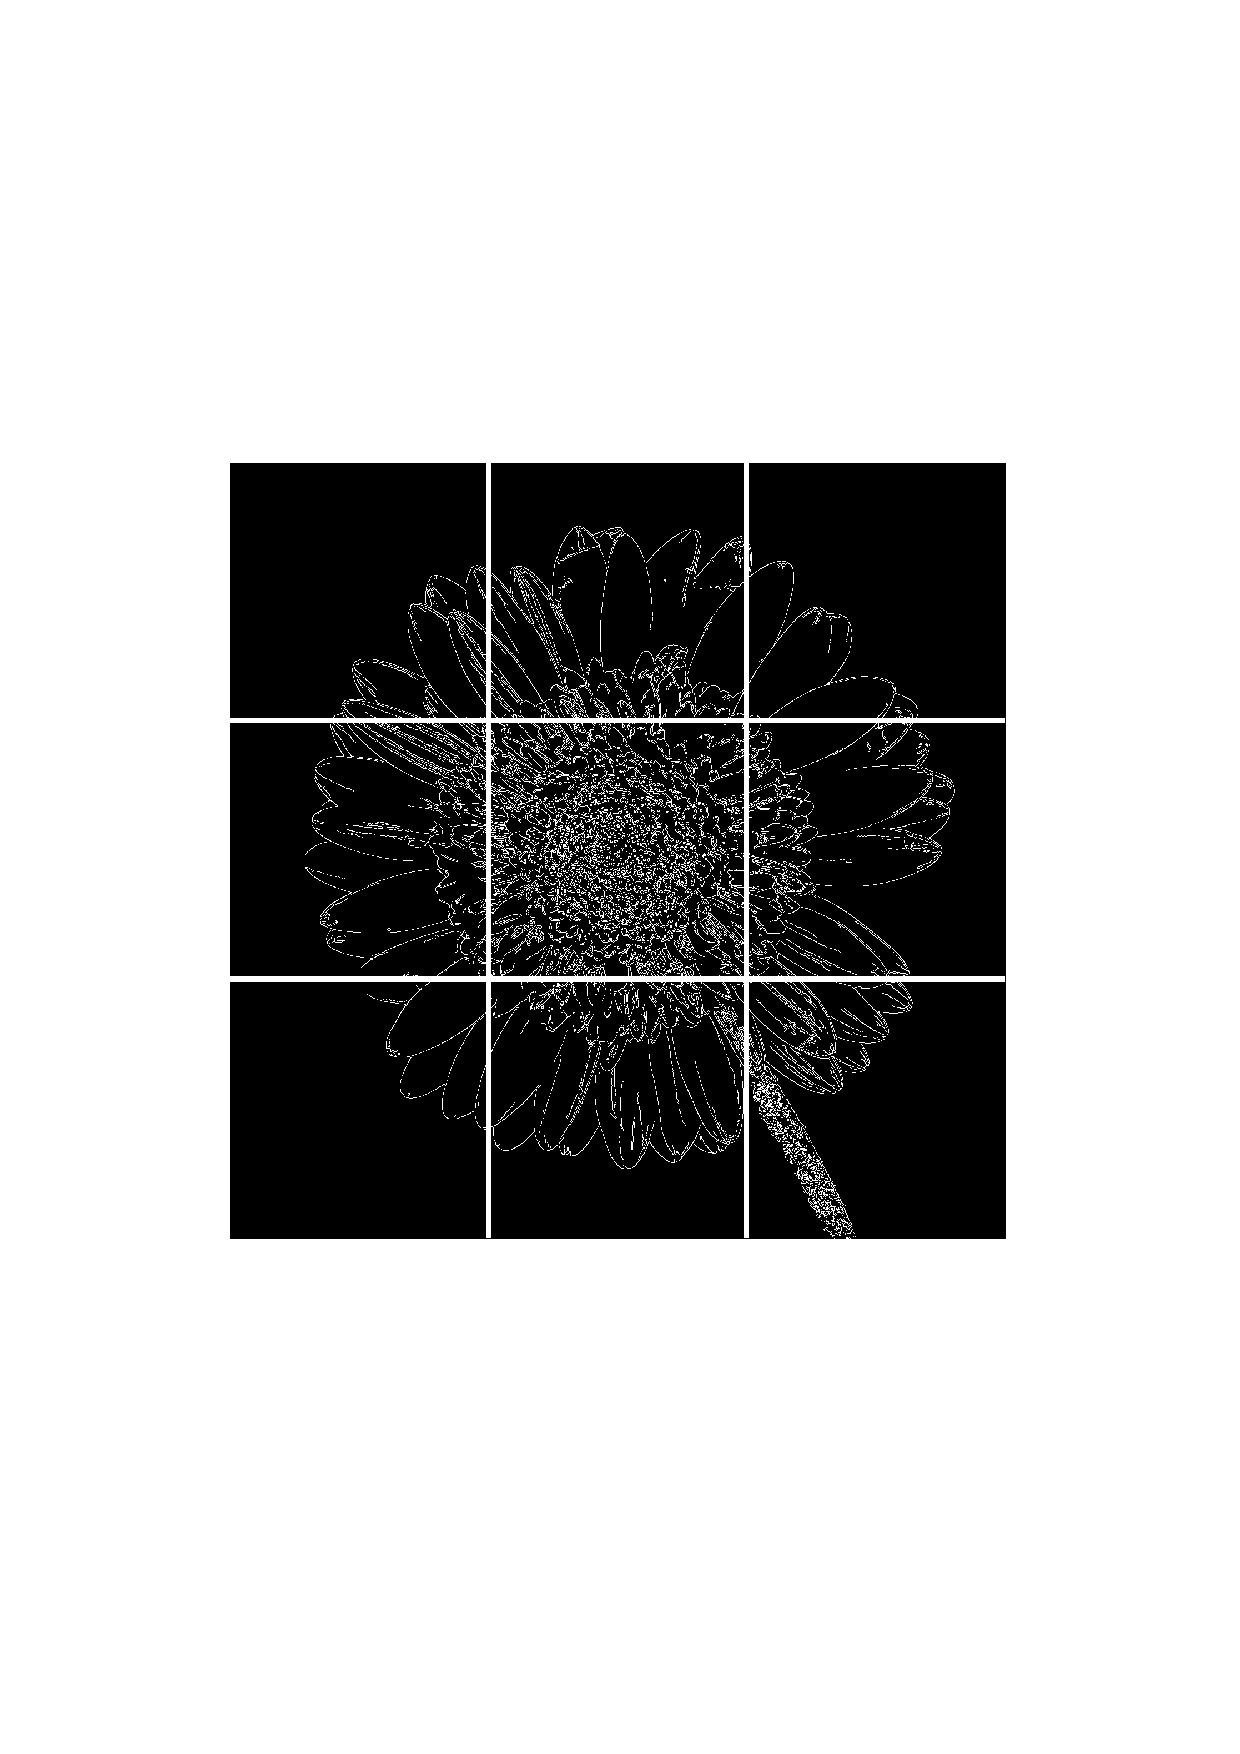
\includegraphics[scale=0.4]{img/gridEdgesFlower}   
\end{center}
\end{figure}
%\textbf{add reference to opencv somewhere}


%\subsubsection{Weibull, this subsubsubsection can be made normal text, but we can do that later}
%The contrast of natural image statistics has been shown to conform to Weibull-shaped probability distributions \cite{Weibull_physical}. Furthermore, when images do not adhere to this distribution, the images in question are mashups of multiple sub-images which themselves do conform to the Weibull distribution. In addition to this property of natural images, it has been proposed that the parameters for the Weibull distribution form a basis for the description of texture in images \cite{Weibull_6}. There is indeed evidence that the human visual system is capable of approximating the parameters of the Weibull distribution \cite{Weibull_brain}. Last the two most important parameters of the Weibull distribution, when it comes to natural images have a straight forward interpretation, the shape parameter the describes the resemblance to other probability distribution, from a power-law to the normal distribution, where the scale describes the how wide the distribution is. Therefore we included the maximum likelihood estimation of the Weibull-distribution for contrast of the image as used for \cite{Weibull_6} in our Feature extraction toolbox, unfortunately this seemed to give unstable results, therefore we later eliminated it. 

\paragraph{\textit{Cognitively-inspired features}\label{proposed-cognitive}}
One of the more recent trends in computer vision research in the pursuit of human-like capability is the coupling of cognition and vision into cognitive computer vision. The term cognitive computer vision has been introduced with the aim of achieving more robust, resilient, and adaptable computer vision systems by endowing them with a cognitive faculty: the ability to learn, adapt, weigh alternative solutions, and develop new strategies for analysis and interpretation.

Recent studies focused on computational models of focal visual attention. Attention has been seen to influences the processing of visual information even in the earliest areas of primate visual cortex. Even more, it has been discovered that the interaction of bottom-up sensory information and top-down attentional influences creates an integrated \textit{saliency map}, that can be defined as a topographic representation of relative stimulus strength and behavioral relevance across visual space \cite{Saliency_WWHW}. This map enables the visual system to integrate large amounts of information, even from outside the fovea, because it provides an efficient coding scheme for the potentially most relevant information in the sensory input. 
An important model based on this theory is the one provided by Itti, Koch and Niebur \cite{Itti_review}\cite{Itti_model}. The model tries to mimic the properties of primate early vision. Despite its simple architecture the model is capable of strong performance with complex natural scene.
The model work as follow: an input image is decomposed through several pre-attentive feature detection mechanisms which operate in parallel channels over the entire visual scene, and four conspicuity maps (color, orientation, intensity and skin) are created. After few different intermediate steps, the model finally combines the four conspicuity maps into a unique saliency map. 

Til now the saliency map has been used as information channel in scene understanding and object recognition. In this reasearch, image features have extracted from the map and then used in the classification and visualization task. Features that have been extracted from those maps are: \textit{Shannon entropy} of the five maps, \textit{Standard deviation} of the distribution of attention in the saliency map, \textit{Location} of the most salient points (defined as the centers of the most salient regions) and \textit{Skin intensity} of the skin map. Skin is not a default channel in the Itti's model, but it has been found out to be really interesting and useful in devianART to distinguish artists and artworks, where there is a huge presence of photographer that create nude art. 


\begin{figure}[h!]
\centering
\subfigure[]{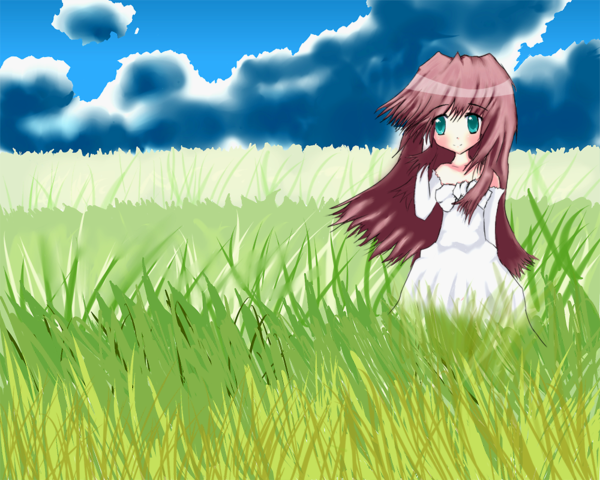
\includegraphics[scale=0.135]{Saliency_images/A_landscape_pic_with_a_loli_bg_by_CroireIgeen.png}\label{fig:saliencyimg1}}
\subfigure[]{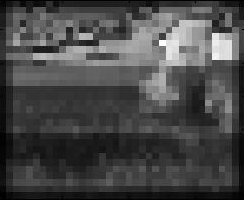
\includegraphics[scale=0.33]{Saliency_images/color.PNG}\label{fig:saliencyimgc1}}
\subfigure[]{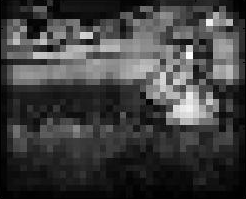
\includegraphics[scale=0.33]{Saliency_images/intensity.PNG}\label{fig:saliencyimgc2}}
\subfigure[]{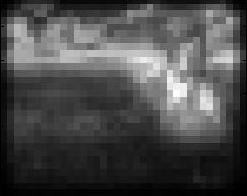
\includegraphics[scale=0.33]{Saliency_images/orientation.PNG}\label{fig:saliencyimgc3}}
\subfigure[]{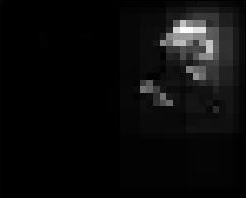
\includegraphics[scale=0.33]{Saliency_images/skin.PNG}\label{fig:saliencyimgc4}}
\subfigure[]{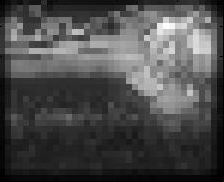
\includegraphics[scale=0.36]{Saliency_images/sm.PNG}\label{fig:ex_saliencymap}}

\caption{Example of saliency maps. (f) shows the final saliency map, while (b), (c), (d) and (e) show the conspicuity maps for color, intensity, orientation and skin respectively.}
\end{figure}


\subsubsection{Classification}

%REVIEW THIS PART!!!
%- FOCUS ON DESCRIBING WHY WE NEED TO CLASSIFY IN OUR PROJECT
%- WHICH CLASSIFIER WE USE AND FOR WHAT REASONS (WE CAN REFER TO SOME PAPERS ////////////////////////// THAT SHOW RESULTS IN VISUAL CLASSIFICATION)
%- EXPLAIN THE EVALUATION MEASURE USED (introduce precision and recall, but they are intermediate measure used to compute the F-Measure!!! P&R never appear in the final results)
%- INTRODUCE THE IDEA OF A DATASET WITHOUT GROUND TRUTH AND WITH THE NEED OF USING 5-FOLD CROSS VALIDATION (check the paper I sent you! ;) )
%- SAY SOMETHING ABOUT FEATURE SELECTION AND HOW WE DO IT! (refer to the description above!! remember feature extraction and classification are in the SAME section and they work together)
%- HOPE THOSE INFORMATION CAN BE USEFUL! ;)

The most important aspect in this project is to describe images, artists or categories using the features that were extracted.
In this approach, classifiers are used to give a performance score to a set of features that is used to either describe an artist or a category.

\paragraph{Data normalization}

Classifiers improve their classification performance when the dataset that is used is normalized.
In this case every extracted feature in the dataset has a different value range, it is important to translate all the different ranges to one defined value range so that the data is normalized.

\begin{equation}
\label{minmax}
y_n=\frac{x_n - \max(x_n)}{\max(x_n)-\min(x_n)} * (B-A)
\end{equation}

Equation \ref{minmax} shows the Min/Max normalization that was used to normalize the data in our approach.
In this equation $A$ and $B$ represents the range [$A$,$B$] where the values are normalized to.
$x$ represents the unnormalized values of feature $n$ whereas $y$ represents the normalized values of feature $n$.

\paragraph{Classifiers}
In our approach, four different classifiers were incorporated to calculate the performance of a set of features.
All classifiers were chosen based on their performance in earlier work except for the Nearest Mean classifier.

The \textit{k-Nearest Neighbour}~\cite{korn1996fast} classifies an artwork based on the training examples that are close to it.
The euclidian distance is used here to measure how far a training example is located from the artwork.

The \textit{Naive Bayes}~\cite{keren2003recognizing} first divides the value range for each feature in $n$ bins.
It then counts the frequency of a training example for each of the classes in every bin and uses that to classify an artwork belonging to the class that gives the maximum posterior probability.

The \textit{Nearest Mean} classifies an artwork based on the euclidian distance to the mean of a class.
The classifier was chosen because it might give a high performance for when the right features are used to describe a class.
This is because the right features of a class will make the artwork of that class cluster.

At last the \textit{Support Vector Machine}~\cite{chapelle1999svms} classifies an artwork using a model created with training examples.
The model represents the training examples in a way that separates the two classes by a clear gap that is as wide as possible.
The artwork is classified by the model based on which side of the gap they fall on.

\paragraph{Feature Selection}
The classifiers are used in our approach to compute the performance score of a set of features.
On the other hand a feature selection algorithm is used to extract a set of features out of all the features that were pre-computed.
This is important because we want to have the smallest set of features to describe a class.

The feature selection in our approach starts by selecting the most informative feature and for each step iteratively adds the next most informative feature to it in a greedy fashion.

\begin{equation}
\label{featureselect}
F := F \cup f, where f: \max{J(f_i)} \wedge f_i \epsilon F
\end{equation}

Formula \ref{featureselect} is a formally written representation of this algorithm.
In this formula, $F$ represents the entire feature set, $f$ one single feature and $J$ the criterion that is used to define if a feature is informative.

The inter-intra distance is used as the criterion to define if a feature is informative.
This criterion works by measuring the inner-scatter of a class over a feature and measures it against the scatter of that class around the average of the feature.
For a two class problem like in our approach the inter-intra distance can be written as:

\begin{equation}
\label{interintra}
J = \frac{|m_1-m_2|}{\sqrt(s^2_1 + s^2_2)}
\end{equation}

In this equation $m_1$ and $m_2$ are the average mean of class 1 and class 2, $s_1$ and $s_2$ are the standard deviations of those classes.
This equation is also equivalent to the Fisher criterion~\cite{malina1981extended}.

\paragraph{Performance measures}
A performance measure is needed to assign a performance score to a set of features.
Because our approach requires the need of classifiers, it is arbitrary that the performance measure is the same as the evaluation measure of the classifier.

Every prediction of the classifier is labeled into one of the following four types,
depending on whether or not the classification was correct:

\begin{tabular}{r|c|c|}
\multicolumn{1}{r}{}
 &  \multicolumn{1}{c}{predicted positive}
 & \multicolumn{1}{c}{predicted negative} \\
\cline{2-3}
positive & \textbf{tp} (true positive) & \textbf{fp} (false positive) \\
\cline{2-3}
negative & \textbf{fn} (false negative) & \textbf{tn} (true negative) \\
\cline{2-3}
\end{tabular}

With these standard classification measures two more evaluation measures can be computed from it.
These are the precision and the recall.
The $precision$ is defined as the number of relevant artwork correctly classified as positive divided by the total number of positive classified artwork.

\begin{equation}
Precision = \frac{tp}{tp + fp}
\end{equation}

The $recall$ is defined as the number of relevant artwork correctly classified as positive divided by the total number of positive examples in the dataset.

\begin{equation}
Recall = \frac{tp}{tp + fn}
\end{equation}

The precision and recall are measures that are used to compute the $F-measure$.
This measure is the weighted harmonic mean of the precision and recall and can be defined as:

\begin{equation}
F_\beta = \frac{(1+\beta)^2 (Precision * Recall)}{(\beta ^2 * Precision) + Recall}
\end{equation}

In our case we use $\beta$=1 which means that the precision and recall are evenly weighted.
